% Options for packages loaded elsewhere
\PassOptionsToPackage{unicode}{hyperref}
\PassOptionsToPackage{hyphens}{url}
%
\documentclass[
]{article}
\usepackage{amsmath,amssymb}
\usepackage{iftex}
\ifPDFTeX
  \usepackage[T1]{fontenc}
  \usepackage[utf8]{inputenc}
  \usepackage{textcomp} % provide euro and other symbols
\else % if luatex or xetex
  \usepackage{unicode-math} % this also loads fontspec
  \defaultfontfeatures{Scale=MatchLowercase}
  \defaultfontfeatures[\rmfamily]{Ligatures=TeX,Scale=1}
\fi
\usepackage{lmodern}
\ifPDFTeX\else
  % xetex/luatex font selection
\fi
% Use upquote if available, for straight quotes in verbatim environments
\IfFileExists{upquote.sty}{\usepackage{upquote}}{}
\IfFileExists{microtype.sty}{% use microtype if available
  \usepackage[]{microtype}
  \UseMicrotypeSet[protrusion]{basicmath} % disable protrusion for tt fonts
}{}
\makeatletter
\@ifundefined{KOMAClassName}{% if non-KOMA class
  \IfFileExists{parskip.sty}{%
    \usepackage{parskip}
  }{% else
    \setlength{\parindent}{0pt}
    \setlength{\parskip}{6pt plus 2pt minus 1pt}}
}{% if KOMA class
  \KOMAoptions{parskip=half}}
\makeatother
\usepackage{xcolor}
\usepackage[margin=1in]{geometry}
\usepackage{color}
\usepackage{fancyvrb}
\newcommand{\VerbBar}{|}
\newcommand{\VERB}{\Verb[commandchars=\\\{\}]}
\DefineVerbatimEnvironment{Highlighting}{Verbatim}{commandchars=\\\{\}}
% Add ',fontsize=\small' for more characters per line
\usepackage{framed}
\definecolor{shadecolor}{RGB}{248,248,248}
\newenvironment{Shaded}{\begin{snugshade}}{\end{snugshade}}
\newcommand{\AlertTok}[1]{\textcolor[rgb]{0.94,0.16,0.16}{#1}}
\newcommand{\AnnotationTok}[1]{\textcolor[rgb]{0.56,0.35,0.01}{\textbf{\textit{#1}}}}
\newcommand{\AttributeTok}[1]{\textcolor[rgb]{0.13,0.29,0.53}{#1}}
\newcommand{\BaseNTok}[1]{\textcolor[rgb]{0.00,0.00,0.81}{#1}}
\newcommand{\BuiltInTok}[1]{#1}
\newcommand{\CharTok}[1]{\textcolor[rgb]{0.31,0.60,0.02}{#1}}
\newcommand{\CommentTok}[1]{\textcolor[rgb]{0.56,0.35,0.01}{\textit{#1}}}
\newcommand{\CommentVarTok}[1]{\textcolor[rgb]{0.56,0.35,0.01}{\textbf{\textit{#1}}}}
\newcommand{\ConstantTok}[1]{\textcolor[rgb]{0.56,0.35,0.01}{#1}}
\newcommand{\ControlFlowTok}[1]{\textcolor[rgb]{0.13,0.29,0.53}{\textbf{#1}}}
\newcommand{\DataTypeTok}[1]{\textcolor[rgb]{0.13,0.29,0.53}{#1}}
\newcommand{\DecValTok}[1]{\textcolor[rgb]{0.00,0.00,0.81}{#1}}
\newcommand{\DocumentationTok}[1]{\textcolor[rgb]{0.56,0.35,0.01}{\textbf{\textit{#1}}}}
\newcommand{\ErrorTok}[1]{\textcolor[rgb]{0.64,0.00,0.00}{\textbf{#1}}}
\newcommand{\ExtensionTok}[1]{#1}
\newcommand{\FloatTok}[1]{\textcolor[rgb]{0.00,0.00,0.81}{#1}}
\newcommand{\FunctionTok}[1]{\textcolor[rgb]{0.13,0.29,0.53}{\textbf{#1}}}
\newcommand{\ImportTok}[1]{#1}
\newcommand{\InformationTok}[1]{\textcolor[rgb]{0.56,0.35,0.01}{\textbf{\textit{#1}}}}
\newcommand{\KeywordTok}[1]{\textcolor[rgb]{0.13,0.29,0.53}{\textbf{#1}}}
\newcommand{\NormalTok}[1]{#1}
\newcommand{\OperatorTok}[1]{\textcolor[rgb]{0.81,0.36,0.00}{\textbf{#1}}}
\newcommand{\OtherTok}[1]{\textcolor[rgb]{0.56,0.35,0.01}{#1}}
\newcommand{\PreprocessorTok}[1]{\textcolor[rgb]{0.56,0.35,0.01}{\textit{#1}}}
\newcommand{\RegionMarkerTok}[1]{#1}
\newcommand{\SpecialCharTok}[1]{\textcolor[rgb]{0.81,0.36,0.00}{\textbf{#1}}}
\newcommand{\SpecialStringTok}[1]{\textcolor[rgb]{0.31,0.60,0.02}{#1}}
\newcommand{\StringTok}[1]{\textcolor[rgb]{0.31,0.60,0.02}{#1}}
\newcommand{\VariableTok}[1]{\textcolor[rgb]{0.00,0.00,0.00}{#1}}
\newcommand{\VerbatimStringTok}[1]{\textcolor[rgb]{0.31,0.60,0.02}{#1}}
\newcommand{\WarningTok}[1]{\textcolor[rgb]{0.56,0.35,0.01}{\textbf{\textit{#1}}}}
\usepackage{graphicx}
\makeatletter
\newsavebox\pandoc@box
\newcommand*\pandocbounded[1]{% scales image to fit in text height/width
  \sbox\pandoc@box{#1}%
  \Gscale@div\@tempa{\textheight}{\dimexpr\ht\pandoc@box+\dp\pandoc@box\relax}%
  \Gscale@div\@tempb{\linewidth}{\wd\pandoc@box}%
  \ifdim\@tempb\p@<\@tempa\p@\let\@tempa\@tempb\fi% select the smaller of both
  \ifdim\@tempa\p@<\p@\scalebox{\@tempa}{\usebox\pandoc@box}%
  \else\usebox{\pandoc@box}%
  \fi%
}
% Set default figure placement to htbp
\def\fps@figure{htbp}
\makeatother
\setlength{\emergencystretch}{3em} % prevent overfull lines
\providecommand{\tightlist}{%
  \setlength{\itemsep}{0pt}\setlength{\parskip}{0pt}}
\setcounter{secnumdepth}{5}
\setcounter{section}{-1}
\usepackage{fvextra}
\DefineVerbatimEnvironment{Highlighting}{Verbatim}{
  showspaces = false,
  showtabs = false,
  breaklines,
  commandchars=\\\{\}
}

\usepackage{bookmark}
\IfFileExists{xurl.sty}{\usepackage{xurl}}{} % add URL line breaks if available
\urlstyle{same}
\hypersetup{
  pdftitle={QRM II Graded Assignment (2), Period 1 2025},
  pdfauthor={Fill in your group number and names here},
  hidelinks,
  pdfcreator={LaTeX via pandoc}}

\title{QRM II Graded Assignment (2), Period 1 2025}
\usepackage{etoolbox}
\makeatletter
\providecommand{\subtitle}[1]{% add subtitle to \maketitle
  \apptocmd{\@title}{\par {\large #1 \par}}{}{}
}
\makeatother
\subtitle{Material by Sjoerd van Alten and Klervie Toczé}
\author{Fill in your group number and names here}
\date{12-09-2025}

\begin{document}
\maketitle

\section{Introduction}\label{introduction}

This assignment is to be completed in groups of 3-4. Further, all
students in your group need to be assigned to the same R tutorial group
(Friday's tutorial). You can sign yourself up for a group on Canvas.
Please do so
\textbf{before the start of your first R tutorial on Friday September 5th.}
You can use the Discussion Board in Canvas if you do not have a group
yet or if your group is incomplete.

The assignment has 5 parts, and each part corresponds to the course
material of that week (with the exclusion of week 6, for which there is
no R programming material).

You are supposed to hand in these assignments on Canvas at the following
dates:

\begin{itemize}
\tightlist
\item
  \textbf{Deadline 1} \emph{Thursday September 25th, at 23:59pm}: you
  are supposed to hand in weeks 1, 2, and 3 of this assignment. This
  will determine 18\% of your overall course grade
\item
  \textbf{Deadline 2} \emph{Thursday October 9th, at 23:59pm}: you are
  supposed to hand in weeks 4, and 5 of this assignment. This will
  determine 12\% of your overall course grade
\end{itemize}

The R tutorials (each Friday) will consist of two halves. During the
first half, you will discuss the tutorial exercises. These can be
downloaded separately from Canvas. During the second half, you can work
on this graded assignment within your own group. The purpose is that you
find out how to work with R for doing statistical analyses by yourself.
The tutorial exercises are meant to teach you basic commands to get you
started, but to answer the problem sets in this assignment, you might
need to research your own solutions, and use functions and commands not
described in the tutorial exercises. Learning how to solve your own
research problems is integral part of learning R. When you and your
group get stuck on how to approach an exercise, the hierarchy in finding
your way is as follows:

\begin{itemize}
\tightlist
\item
  use the concepts from the tutorial exercises;
\item
  use the cheat sheets available on Canvas;
\item
  use Google, YouTube, StackOverflow, or another website;
\item
  ask the teacher.
\end{itemize}

The use of generative AI is \textbf{not} permitted and may result in a
grade of 0. See the AI protocol in the course manual for details.

To answer the assignment, you can simply fill out this R markdown
document. There are designated places which you can fill with R code.
There are also designated spaces for you to answer each question. Often,
the structure of an answer will be as follows. First, you type the R
code in the designated box. This will show how you analyzed the data to
get the answer to the question. Below the box for the R code, you will
then summarize your answer to the question, i.e.~what are the
conclusions that you draw from the data analysis?

When handing in, you are supposed to submit this .Rmd file, and a
knitted version of this document. You can knit this document to pdf,
word, or html. Knitting to pdf requires you to have a .tex distribution
installed on your computer. Knitting to Word requires you to have Word
installed.

The exercises are designed such that you should be able to finish the
majority of them during the tutorial each week. If you are not able to
finish them fully during that time, you are expected to work on it in
your own time using the computers on campus or your own device. It is
best to meet as a group in-person when working together. If you want to
work remotely, github is a good platform to guarantee smooth
collaboration. Alternatively, you can email this .Rmd file back and
forth to one another as a group, but this is not recommended as it is
more cumbersome.

We encourage you to keep your code blocks, printing statements, and
final answers, as short as possible. In any case, there is a page limit
of 6 pages per week, which encompasses the total length of this document
which consists of the questions, your coding lines, and your answers.
When your answers to questions of the respective week exceed this page
limit, they will not be graded, resulting in zero points.

Each week consists of 1, 2, or 3 subquestions. The total amount of
points you can earn per week is 20 points.

\section{Week 1}\label{week-1}

\begin{enumerate}
\def\labelenumi{\arabic{enumi}.}
\tightlist
\item
  Find the dataset ``movies1.tsv'' on Canvas. Describe your data set:
  How many observations does it have. How many variables are there? How
  many subjects? What consists of a subject? \textbf{[4 points]}
\end{enumerate}

\begin{Shaded}
\begin{Highlighting}[]
\NormalTok{movies }\OtherTok{\textless{}{-}} \FunctionTok{read.table}\NormalTok{(}\StringTok{"movies1.tsv"}\NormalTok{, }\AttributeTok{header=}\ConstantTok{TRUE}\NormalTok{)}

\FunctionTok{head}\NormalTok{(movies)}
\end{Highlighting}
\end{Shaded}

\begin{verbatim}
##   index  budget
## 1  1773 2.7e+07
## 2  2540 1.5e+07
## 3  1174 4.0e+07
## 4  3262 0.0e+00
## 5  4324 0.0e+00
## 6   214 1.2e+08
##                                                                            keywords
## 1                                        fbi island serial killer series of murders
## 2                                 fire winter santa claus snow storm christmas tree
## 3 police sequel police officer brother-in-law brother-in-law relationship black men
## 4                  masseuse thanksgiving party romance mother daughter relationship
## 5                                                               christian film food
## 6                         u.s. air force grocery jamaican meteorologist rescue boat
##   original_language               title popularity release_date   revenue
## 1                en         Mindhunters  17.193659   2004-05-07  21148829
## 2                en             Krampus  31.565117   2015-11-26  61548707
## 3                en        Ride Along 2  25.136082   2016-01-14 124827316
## 4                en         Enough Said  14.969093   2013-09-18  25288872
## 5                en Faith Like Potatoes   0.147886   2006-10-27         0
## 6                en   The Perfect Storm  25.752118   2000-03-15 325756637
##   runtime vote_average vote_count    genre release_year release_month
## 1     106          6.3        333 Thriller         2004             5
## 2      98          5.9        584   Comedy         2015            11
## 3     102          6.1        555   Comedy         2016             1
## 4      93          6.6        348    Drama         2013             9
## 5      97          6.0          9    Drama         2006            10
## 6     130          6.2        597    Drama         2000             3
##   release_day         first_actor first_actor_gender director_first_name
## 1           7             LL Cool               <NA>               Renny
## 2          26          Adam Scott               male             Michael
## 3          14          Kevin Hart               male                 Tim
## 4          18 Julia Louis-Dreyfus             female              Nicole
## 5          27    Frank Rautenbach               male             Regardt
## 6          15      George Clooney               male            Wolfgang
##   director_gender
## 1            male
## 2            male
## 3            male
## 4          female
## 5            <NA>
## 6            male
\end{verbatim}

\begin{Shaded}
\begin{Highlighting}[]
\FunctionTok{ncol}\NormalTok{(movies)}
\end{Highlighting}
\end{Shaded}

\begin{verbatim}
## [1] 19
\end{verbatim}

\begin{Shaded}
\begin{Highlighting}[]
\FunctionTok{nrow}\NormalTok{(movies)}
\end{Highlighting}
\end{Shaded}

\begin{verbatim}
## [1] 505
\end{verbatim}

\textbf{Your Answer}

We conclude that the data set has 19 variables and 505 subjects. Every
subject consists of a unique movie.

\begin{enumerate}
\def\labelenumi{\arabic{enumi}.}
\setcounter{enumi}{1}
\tightlist
\item
  Which of the following types of variables are present in your data
  set? (i) nominal; (ii) ordinal; (iii); interval; (iv) ratio. If
  present, name one example of such a variable present in your data set.
  \textbf{[4 points]}
\end{enumerate}

\begin{Shaded}
\begin{Highlighting}[]
\CommentTok{\#WRITE YOUR CODE HERE}
\FunctionTok{str}\NormalTok{(movies)}
\end{Highlighting}
\end{Shaded}

\begin{verbatim}
## 'data.frame':    505 obs. of  19 variables:
##  $ index              : int  1773 2540 1174 3262 4324 214 1737 610 2738 963 ...
##  $ budget             : num  2.70e+07 1.50e+07 4.00e+07 0.00 0.00 1.20e+08 2.80e+07 7.00e+07 1.25e+07 4.00e+07 ...
##  $ keywords           : chr  "fbi island serial killer series of murders" "fire winter santa claus snow storm christmas tree" "police sequel police officer brother-in-law brother-in-law relationship black men" "masseuse thanksgiving party romance mother daughter relationship" ...
##  $ original_language  : chr  "en" "en" "en" "en" ...
##  $ title              : chr  "Mindhunters" "Krampus" "Ride Along 2" "Enough Said" ...
##  $ popularity         : num  17.194 31.565 25.136 14.969 0.148 ...
##  $ release_date       : chr  "2004-05-07" "2015-11-26" "2016-01-14" "2013-09-18" ...
##  $ revenue            : num  2.11e+07 6.15e+07 1.25e+08 2.53e+07 0.00 ...
##  $ runtime            : int  106 98 102 93 97 130 108 99 100 99 ...
##  $ vote_average       : num  6.3 5.9 6.1 6.6 6 6.2 5.5 4.4 6 6.2 ...
##  $ vote_count         : int  333 584 555 348 9 597 640 533 210 371 ...
##  $ genre              : chr  "Thriller" "Comedy" "Comedy" "Drama" ...
##  $ release_year       : int  2004 2015 2016 2013 2006 2000 2016 2014 2014 2009 ...
##  $ release_month      : int  5 11 1 9 10 3 2 1 2 9 ...
##  $ release_day        : int  7 26 14 18 27 15 4 10 14 29 ...
##  $ first_actor        : chr  "LL Cool" "Adam Scott" "Kevin Hart" "Julia Louis-Dreyfus" ...
##  $ first_actor_gender : chr  NA "male" "male" "female" ...
##  $ director_first_name: chr  "Renny" "Michael" "Tim" "Nicole" ...
##  $ director_gender    : chr  "male" "male" "male" "female" ...
\end{verbatim}

The chr ones are often nominal, the int ones are ratio and the num ones
are ratio or interval. The ordinal ones are ordered factors, but not in
our data. Nominal: orginal\_language Inverval: popularity Ratio:
vote\_count

\begin{enumerate}
\def\labelenumi{\arabic{enumi}.}
\setcounter{enumi}{2}
\tightlist
\item
  A movie studio wants to know which types of movies give maximal
  profit. Perform the following steps to provide the movie studio with
  an analysis which corresponds to their request:
\end{enumerate}

\begin{enumerate}
\def\labelenumi{\alph{enumi}.}
\tightlist
\item
  Create the variable profits as the revenue of a movie minus its
  budget. Report its mean, median, maximum, and minimum.
  \textbf{[2 points]}
\item
  Which movie has the highest profits in your data set and how much are
  these profits. Which movie has the lowest and how much are its
  profits? If multiple movies have the exact same highest or lowest
  profits, give only one example. \textbf{[2 points]}
\item
  Create a boxplot of the variable profits. Make sure it has an
  appropriate title, and appropriate titles and labels for the x- and
  y-axis. Give Q1, Q2, Q3, and Q4. What does this tell you about the
  nature of making money in the movies industry? \textbf{[2 points]}
\item
  Add a new variable to your data set the log of profits. When creating
  this variable, what happens to movies for which profits is zero or
  negative? What then happens when you calculate the mean of log of
  profits? \textbf{[2 points]}
\item
  For movies that have a profit of zero or less, replace log of profits
  with ``NA''. What is now the mean of log of profits? Create a boxplot
  for log of profits, again with an appropriate title, x- and y-axis
  labels. How does it compare to the boxplot you made under c.)?
  \textbf{[2 points]}
\item
  Create a scatterplot of with the runtime of movies on the x-axis and
  the average vote of movies on the y-axis. What do you conclude from
  the scatterplot? Are movies with a longer runtime considered worse or
  better by the audience, or does the audience not have a preference?
  Why do you think this is the case? \textbf{[2 points]}
\end{enumerate}

For each step, you should provide first all the code you used to answer
the question and then formulate an answer using full sentences.

\emph{Step a}

\begin{Shaded}
\begin{Highlighting}[]
\FunctionTok{library}\NormalTok{(tidyverse)}
\end{Highlighting}
\end{Shaded}

\begin{verbatim}
## -- Attaching core tidyverse packages ------------------------ tidyverse 2.0.0 --
## v dplyr     1.1.4     v readr     2.1.5
## v forcats   1.0.0     v stringr   1.5.1
## v ggplot2   3.5.2     v tibble    3.3.0
## v lubridate 1.9.4     v tidyr     1.3.1
## v purrr     1.0.4     
## -- Conflicts ------------------------------------------ tidyverse_conflicts() --
## x dplyr::filter() masks stats::filter()
## x dplyr::lag()    masks stats::lag()
## i Use the conflicted package (<http://conflicted.r-lib.org/>) to force all conflicts to become errors
\end{verbatim}

\begin{Shaded}
\begin{Highlighting}[]
\NormalTok{movies}\SpecialCharTok{$}\NormalTok{profit }\OtherTok{=}\NormalTok{ movies}\SpecialCharTok{$}\NormalTok{revenue }\SpecialCharTok{{-}}\NormalTok{ movies}\SpecialCharTok{$}\NormalTok{budget}

\NormalTok{movies }\SpecialCharTok{\%\textgreater{}\%}
  \FunctionTok{summarise}\NormalTok{(}\FunctionTok{mean}\NormalTok{(profit),}
            \FunctionTok{median}\NormalTok{(profit),}
            \FunctionTok{min}\NormalTok{(profit),}
            \FunctionTok{max}\NormalTok{(profit))}
\end{Highlighting}
\end{Shaded}

\begin{verbatim}
##   mean(profit) median(profit) min(profit) max(profit)
## 1     63121475        1900000      -9e+07  2550965087
\end{verbatim}

\textbf{Your Answer:}

The mean of the variable profit is 63.121.475 euros. The median of the
variable profit is 1.900.000 euros. the minimum of the variable profit
is -90.000.000 euros the maximum of the variable profit is 2.550.965.087
euros

\emph{Step b}

\begin{Shaded}
\begin{Highlighting}[]
\CommentTok{\#WRITE YOUR CODE HERE}
\NormalTok{max\_profit }\OtherTok{=} \FunctionTok{max}\NormalTok{(movies}\SpecialCharTok{$}\NormalTok{profit)}
\NormalTok{min\_profit }\OtherTok{=} \FunctionTok{min}\NormalTok{(movies}\SpecialCharTok{$}\NormalTok{profit)}

\NormalTok{movies }\SpecialCharTok{\%\textgreater{}\%}
  \FunctionTok{filter}\NormalTok{(profit }\SpecialCharTok{==}\NormalTok{ max\_profit) }\SpecialCharTok{\%\textgreater{}\%}
  \FunctionTok{select}\NormalTok{(title, profit)}
\end{Highlighting}
\end{Shaded}

\begin{verbatim}
##    title     profit
## 1 Avatar 2550965087
\end{verbatim}

\begin{Shaded}
\begin{Highlighting}[]
\NormalTok{movies }\SpecialCharTok{\%\textgreater{}\%}
  \FunctionTok{filter}\NormalTok{(profit }\SpecialCharTok{==}\NormalTok{ min\_profit) }\SpecialCharTok{\%\textgreater{}\%}
  \FunctionTok{select}\NormalTok{(title, profit)}
\end{Highlighting}
\end{Shaded}

\begin{verbatim}
##              title profit
## 1 Mighty Joe Young -9e+07
\end{verbatim}

\textbf{Your Answer:}

The movie with the highest profit is Avatar. Its profit is 2.550.965.087
euros. The movie with the lowest profit is Mighty Joe Young. Its profit
is -90.000.000 euros.

\emph{Step c}

\begin{Shaded}
\begin{Highlighting}[]
\CommentTok{\#WRITE YOUR CODE HERE}
\FunctionTok{boxplot}\NormalTok{(movies}\SpecialCharTok{$}\NormalTok{profit, }
        \AttributeTok{main=}\StringTok{"Variable Profit"}\NormalTok{,}
        \AttributeTok{ylab=}\StringTok{"Profit"}\NormalTok{,}
        \AttributeTok{xlab=}\StringTok{"Movies"}\NormalTok{)}
\end{Highlighting}
\end{Shaded}

\pandocbounded{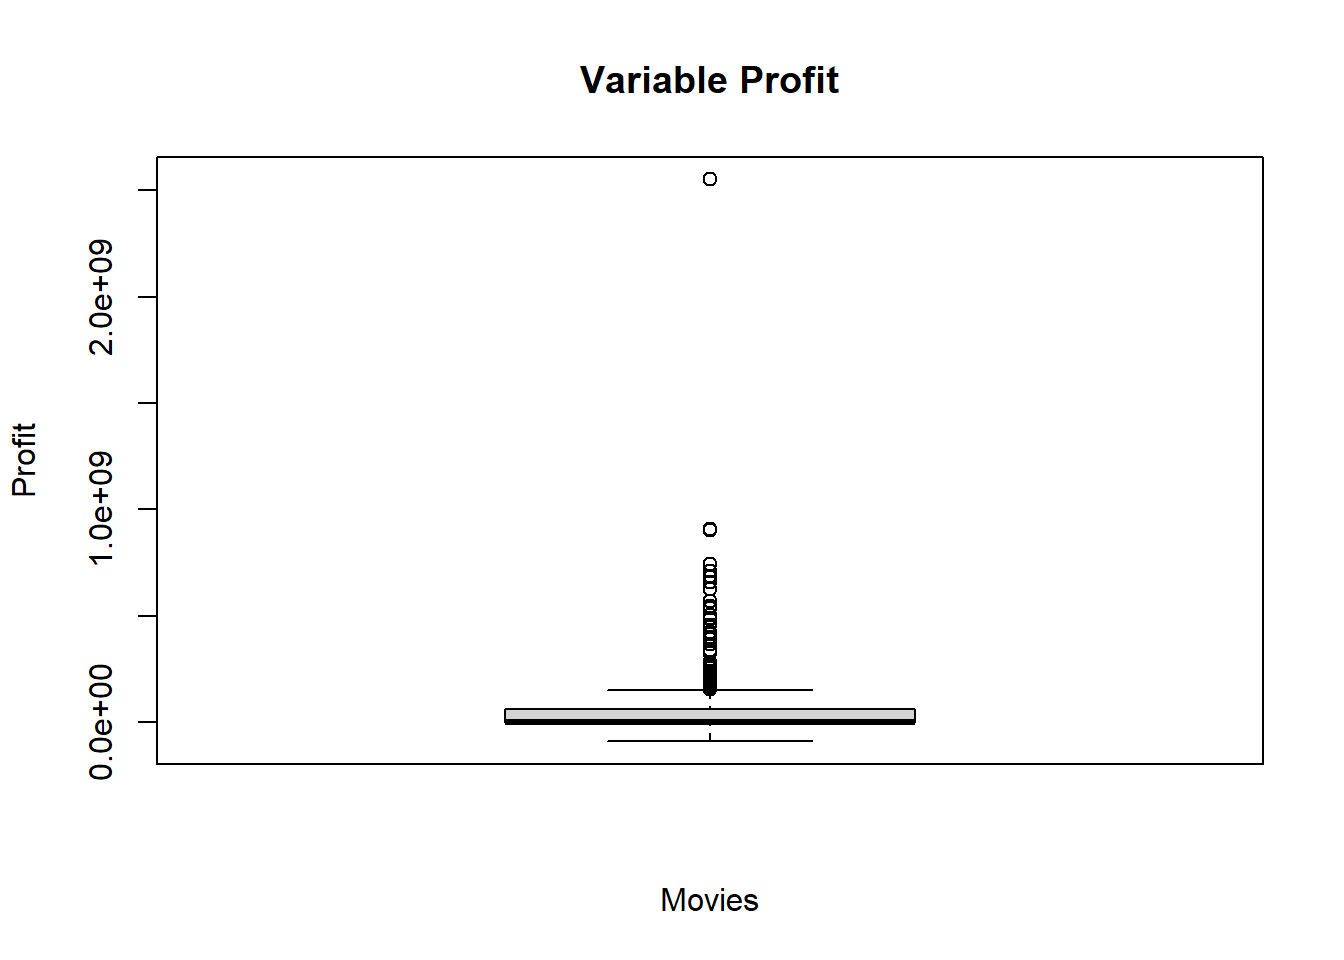
\includegraphics[keepaspectratio]{Assignment2_files/figure-latex/unnamed-chunk-5-1.pdf}}

\begin{Shaded}
\begin{Highlighting}[]
\NormalTok{Q1 }\OtherTok{=} \FunctionTok{quantile}\NormalTok{(movies}\SpecialCharTok{$}\NormalTok{profit, }\FloatTok{0.25}\NormalTok{)}
\NormalTok{Q2 }\OtherTok{=} \FunctionTok{quantile}\NormalTok{(movies}\SpecialCharTok{$}\NormalTok{profit, }\FloatTok{0.50}\NormalTok{)}
\NormalTok{Q3 }\OtherTok{=} \FunctionTok{quantile}\NormalTok{(movies}\SpecialCharTok{$}\NormalTok{profit, }\FloatTok{0.75}\NormalTok{)}
\NormalTok{Q4 }\OtherTok{=} \FunctionTok{max}\NormalTok{(movies}\SpecialCharTok{$}\NormalTok{profit)}

\NormalTok{Q1}
\end{Highlighting}
\end{Shaded}

\begin{verbatim}
## 25% 
##   0
\end{verbatim}

\begin{Shaded}
\begin{Highlighting}[]
\NormalTok{Q2}
\end{Highlighting}
\end{Shaded}

\begin{verbatim}
##     50% 
## 1900000
\end{verbatim}

\begin{Shaded}
\begin{Highlighting}[]
\NormalTok{Q3}
\end{Highlighting}
\end{Shaded}

\begin{verbatim}
##      75% 
## 60514050
\end{verbatim}

\begin{Shaded}
\begin{Highlighting}[]
\NormalTok{Q4}
\end{Highlighting}
\end{Shaded}

\begin{verbatim}
## [1] 2550965087
\end{verbatim}

\begin{Shaded}
\begin{Highlighting}[]
\FunctionTok{boxplot}\NormalTok{(movies}\SpecialCharTok{$}\NormalTok{profit,}
        \AttributeTok{main=}\StringTok{\textquotesingle{}Variable Profit\textquotesingle{}}\NormalTok{,}
        \AttributeTok{ylab=}\StringTok{"Profit"}\NormalTok{,}
        \AttributeTok{xlab=}\StringTok{"Movies"}\NormalTok{,}
        \AttributeTok{outline =} \ConstantTok{FALSE}\NormalTok{)}
\end{Highlighting}
\end{Shaded}

\pandocbounded{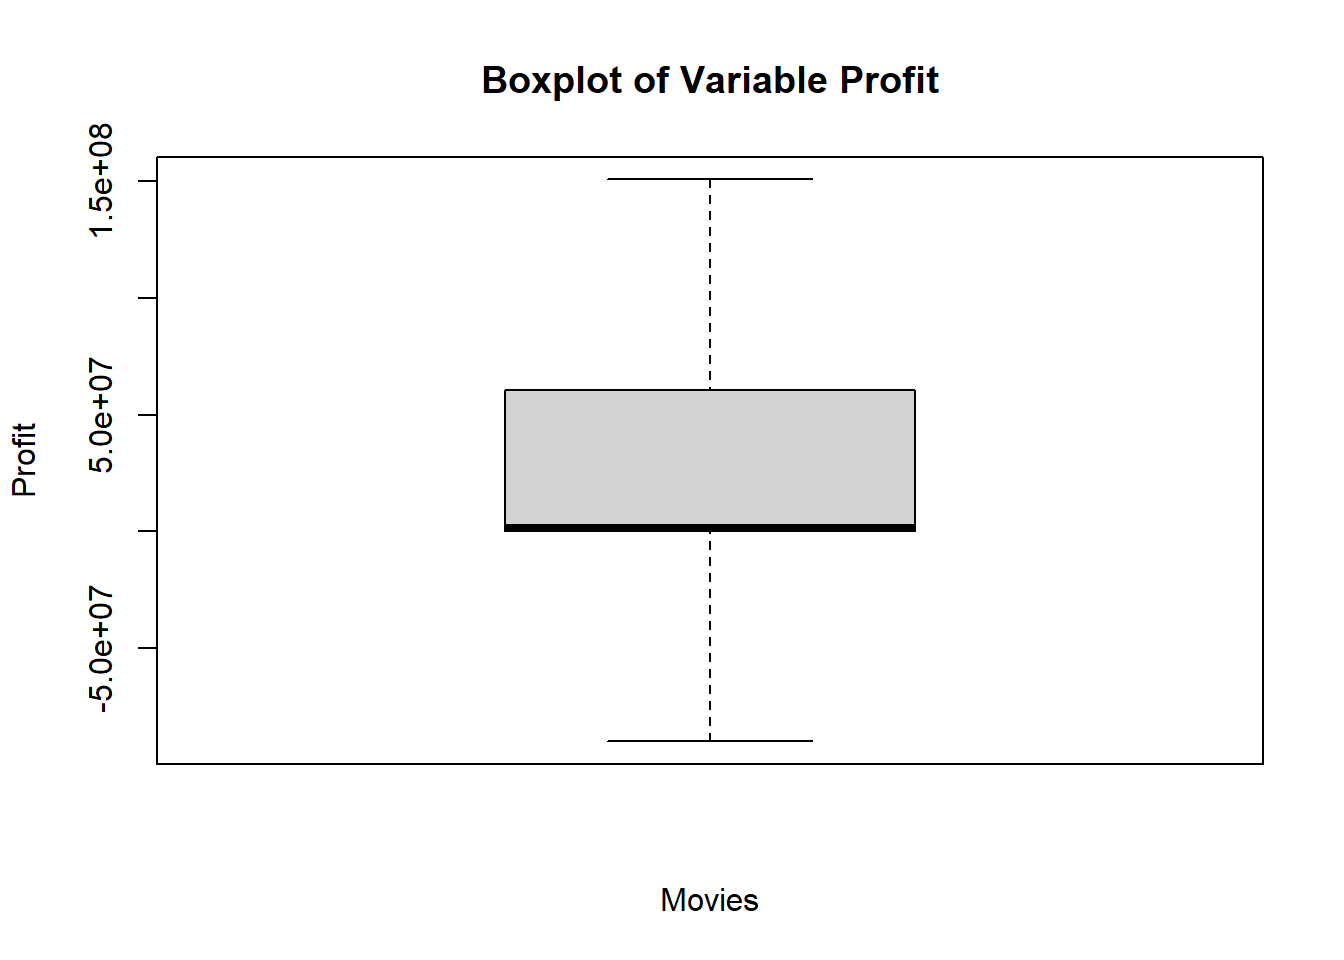
\includegraphics[keepaspectratio]{Assignment2_files/figure-latex/unnamed-chunk-5-2.pdf}}

\textbf{Your Answer:}

We created two boxplots. The first code is for all variable data in the
dataset. The resulting boxplot is very compact with many outliers. In
the second code, which was written to create the boxplot, the outliers
were removed. We did this using the line \#outline = FALSE\#. This
provides a more specific view of the distribution of variable profit.

We calculated the quartiles based on all the data, including the
outliers. These are the quartiles: Q1 = 0 Q2 = 1.900.000 Q3 = 60.514.050
Q4 = 2.550.965.087

This data tells us that the movie industry is a high-risk, high-reward
business, where the majority of films earn little, and profitability is
driven by a small fraction of massive blockbusters.

\emph{Step d}

\begin{Shaded}
\begin{Highlighting}[]
\NormalTok{movies}\SpecialCharTok{$}\NormalTok{log\_profits }\OtherTok{=} \FunctionTok{log}\NormalTok{(movies}\SpecialCharTok{$}\NormalTok{profit)}
\end{Highlighting}
\end{Shaded}

\begin{verbatim}
## Warning in log(movies$profit): NaNs produced
\end{verbatim}

\begin{Shaded}
\begin{Highlighting}[]
\NormalTok{movies }\SpecialCharTok{\%\textgreater{}\%}
  \FunctionTok{summarise}\NormalTok{(}\AttributeTok{mean\_profits =} \FunctionTok{mean}\NormalTok{(log\_profits[}\FunctionTok{is.finite}\NormalTok{(log\_profits)], }\AttributeTok{na.rm =} \ConstantTok{TRUE}\NormalTok{))}
\end{Highlighting}
\end{Shaded}

\begin{verbatim}
##   mean_profits
## 1     17.38094
\end{verbatim}

\textbf{Your Answer:}

All films without profit are converted to -infinity, because the value
of log(0) is not defined for any base of the logarithm All films with a
negative profit are converted to NaN, which means that the result of a
mathematical calculation is not a valid number. This is because the
logarithm is only defined for positive real numbers.

As a result, when calculating the average logarithm of profits, films
with zero or negative profits are excluded from the calculation, as
their logarithm values are undefined. The average then only reflects
films with positive profits, which distorts the result because
loss-making or break-even films are not taken into account.

\emph{Step e}

\begin{Shaded}
\begin{Highlighting}[]
\CommentTok{\#WRITE YOUR CODE HERE}
\NormalTok{movies}\SpecialCharTok{$}\NormalTok{log\_profits[movies}\SpecialCharTok{$}\NormalTok{log\_profits}\SpecialCharTok{\textless{}=}\DecValTok{0}\NormalTok{]}\OtherTok{\textless{}{-}} \ConstantTok{NA}
\NormalTok{movies}\SpecialCharTok{$}\NormalTok{log\_profits[}\FunctionTok{is.nan}\NormalTok{(movies}\SpecialCharTok{$}\NormalTok{log\_profits)] }\OtherTok{\textless{}{-}} \ConstantTok{NA}

\FunctionTok{mean}\NormalTok{(movies}\SpecialCharTok{$}\NormalTok{log\_profits, }\AttributeTok{na.rm =} \ConstantTok{TRUE}\NormalTok{)}
\end{Highlighting}
\end{Shaded}

\begin{verbatim}
## [1] 17.38094
\end{verbatim}

\begin{Shaded}
\begin{Highlighting}[]
\FunctionTok{boxplot}\NormalTok{(movies}\SpecialCharTok{$}\NormalTok{log\_profits,}
        \AttributeTok{main =} \StringTok{"Log of Profits"}\NormalTok{,}
        \AttributeTok{xlab =} \StringTok{"Movies"}\NormalTok{,}
        \AttributeTok{ylab =} \StringTok{"Log of Profits"}\NormalTok{)}
\end{Highlighting}
\end{Shaded}

\pandocbounded{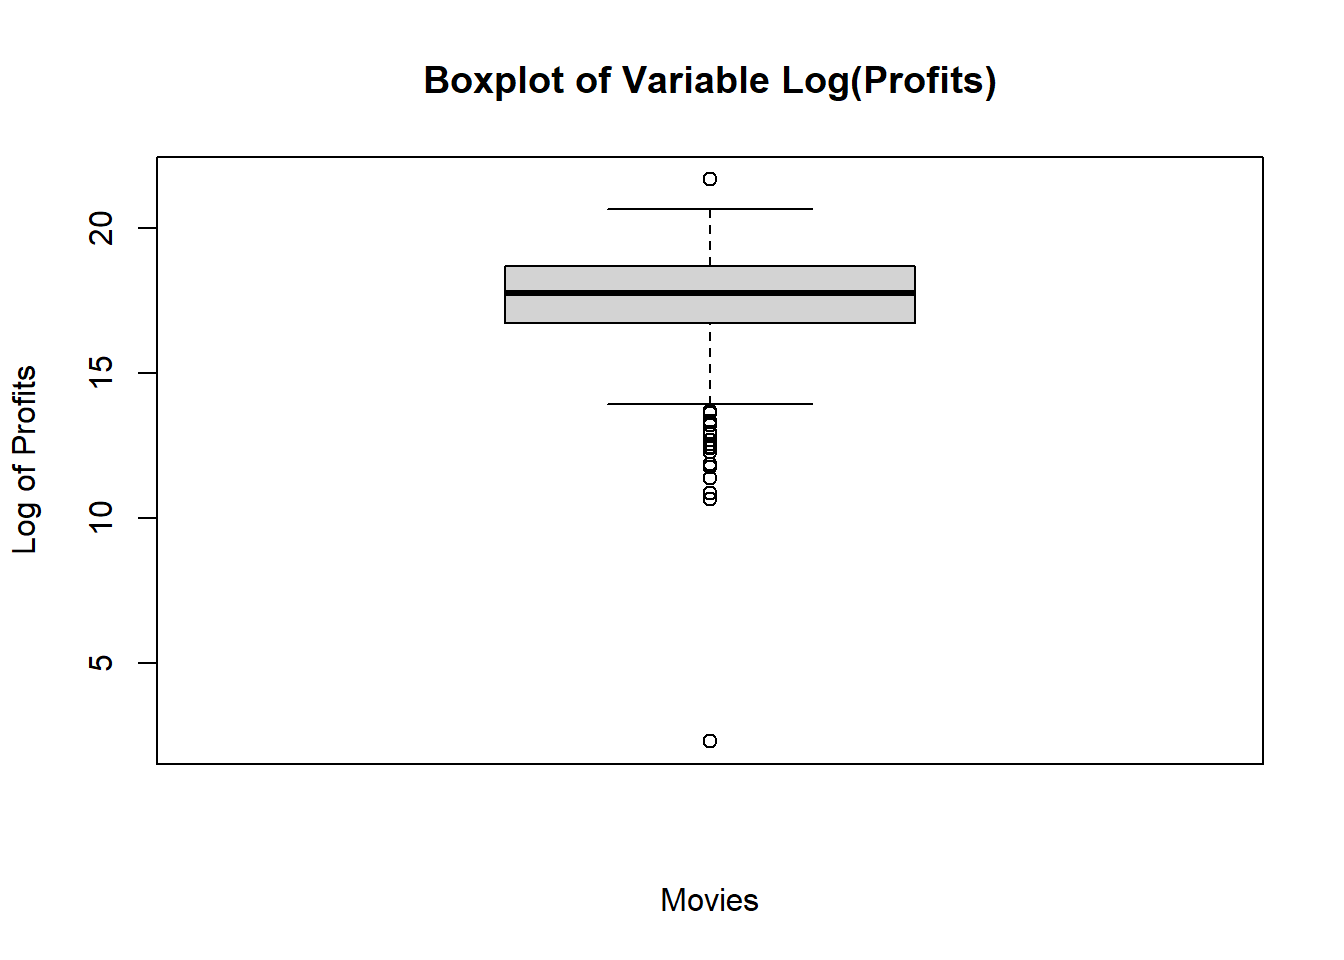
\includegraphics[keepaspectratio]{Assignment2_files/figure-latex/unnamed-chunk-7-1.pdf}}

\textbf{Your Answer:}

Because the values now lie within a more manageable scale, the boxplot
provides more information than in c.~Additionally, all negative values
have been removed from the data, so only positive values are visible in
the boxplot. However, there are still outliers, which can be seen as the
points below the boxplot.

\emph{Step f}

\begin{Shaded}
\begin{Highlighting}[]
\CommentTok{\#WRITE YOUR CODE HERE}
\FunctionTok{ggplot}\NormalTok{(movies, }\FunctionTok{aes}\NormalTok{(}\AttributeTok{x=}\NormalTok{runtime, }\AttributeTok{y=}\NormalTok{vote\_average))}\SpecialCharTok{+}
  \FunctionTok{geom\_point}\NormalTok{()}\SpecialCharTok{+}
  \FunctionTok{geom\_smooth}\NormalTok{(}\AttributeTok{method=}\StringTok{"lm"}\NormalTok{, }\AttributeTok{se=}\NormalTok{T)}
\end{Highlighting}
\end{Shaded}

\begin{verbatim}
## `geom_smooth()` using formula = 'y ~ x'
\end{verbatim}

\begin{verbatim}
## Warning: Removed 1 row containing non-finite outside the scale range
## (`stat_smooth()`).
\end{verbatim}

\begin{verbatim}
## Warning: Removed 1 row containing missing values or values outside the scale range
## (`geom_point()`).
\end{verbatim}

\pandocbounded{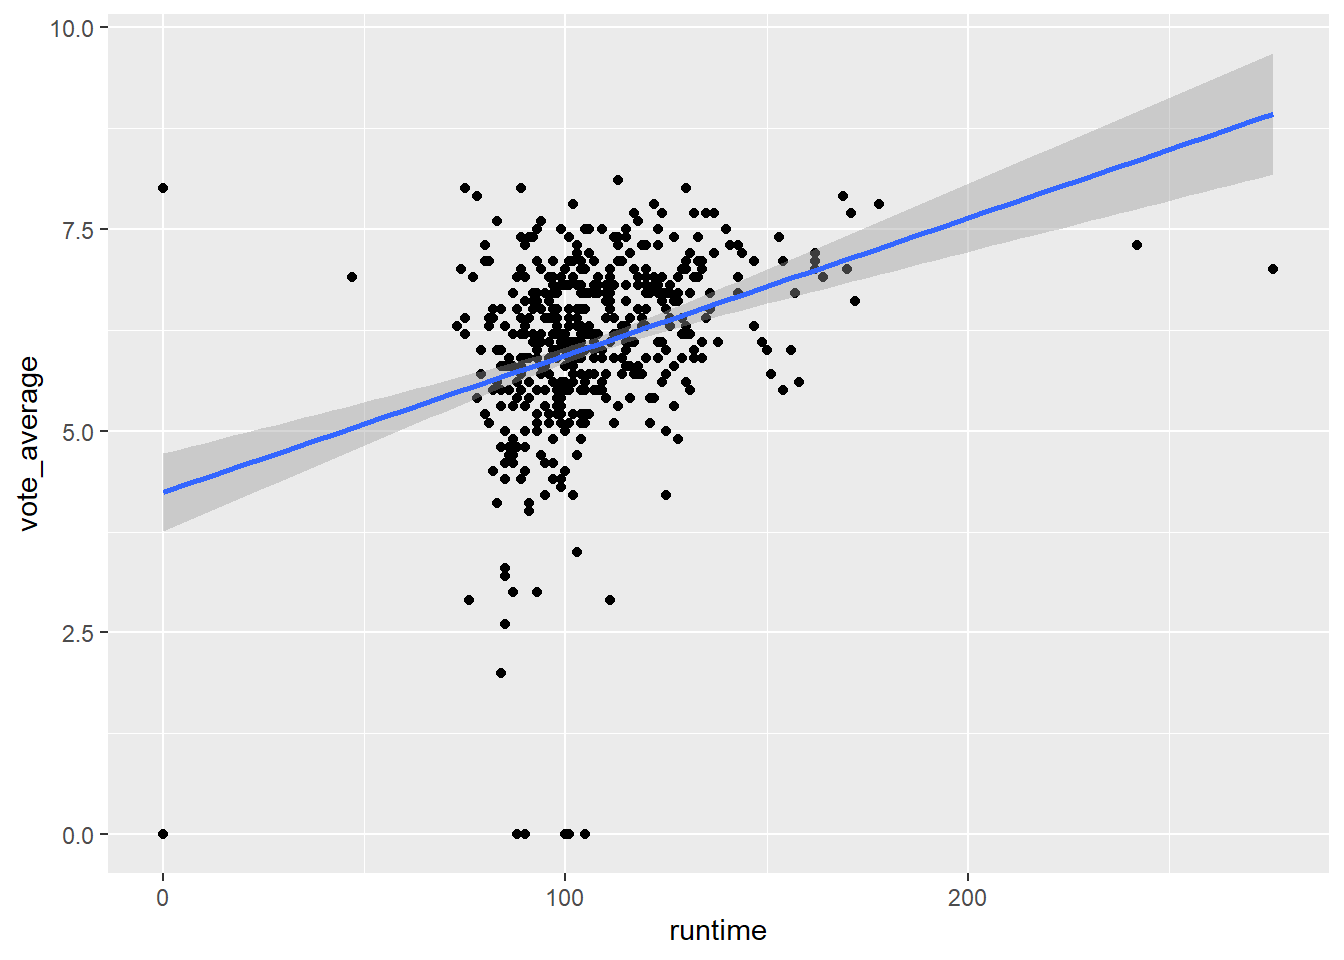
\includegraphics[keepaspectratio]{Assignment2_files/figure-latex/unnamed-chunk-8-1.pdf}}

\textbf{Your Answer:}

The average lies around the 100 minutes, movies with a longer runtome
are considered better.

\section{Week 2}\label{week-2}

1 Is your dataset movies1.tsv the full population, or is it a sample of
a larger population? If the latter, how would you describe the full
population? \textbf{[4 points]}

\begin{Shaded}
\begin{Highlighting}[]
\CommentTok{\#WRITE YOUR CODE HERE}
\end{Highlighting}
\end{Shaded}

\textbf{Your Answer:}

Write your formulated response here.

2

\begin{enumerate}
\def\labelenumi{\alph{enumi}.}
\tightlist
\item
  For which actor in your data set do you observe the most movies?
  \textbf{[2 points]}
\item
  What is the average revenue of the movie in which this actor plays and
  does the revenue lie above or below the revenue of an average movie
  according to your data set? \textbf{[2 points]}\\
\item
  How trustworthy do you consider your conclusion to answer 2b? Use the
  term ``law of large numbers'' in your explanation. \textbf{[2 points]}
\end{enumerate}

\emph{step a}

\begin{Shaded}
\begin{Highlighting}[]
\CommentTok{\#WRITE YOUR CODE HERE}
\NormalTok{actor\_counts }\OtherTok{\textless{}{-}} \FunctionTok{sort}\NormalTok{(}\FunctionTok{table}\NormalTok{(movies}\SpecialCharTok{$}\NormalTok{first\_actor), }\AttributeTok{decreasing =} \ConstantTok{TRUE}\NormalTok{)}
\FunctionTok{head}\NormalTok{(actor\_counts, }\DecValTok{1}\NormalTok{)}
\end{Highlighting}
\end{Shaded}

\begin{verbatim}
## 
## Bruce Willis 
##            7
\end{verbatim}

\textbf{Your Answer:}

Bruce Willis is the actor who plays in the most movies. He plays in 7
movies.

\emph{step b}

\begin{Shaded}
\begin{Highlighting}[]
\CommentTok{\#WRITE YOUR CODE HERE}
\NormalTok{average\_revenue}\OtherTok{\textless{}{-}}\NormalTok{ movies }\SpecialCharTok{\%\textgreater{}\%} 
  \FunctionTok{filter}\NormalTok{(first\_actor}\SpecialCharTok{==}\StringTok{"Bruce Willis"}\NormalTok{) }\SpecialCharTok{\%\textgreater{}\%} 
  \FunctionTok{summarise}\NormalTok{(}\AttributeTok{average\_revenue\_Bruce=}\FunctionTok{mean}\NormalTok{(revenue, }\AttributeTok{na.rm=}\NormalTok{T))}

\FunctionTok{mean}\NormalTok{(movies}\SpecialCharTok{$}\NormalTok{revenue)}
\end{Highlighting}
\end{Shaded}

\begin{verbatim}
## [1] 94815482
\end{verbatim}

\textbf{Your Answer:}

The average revenue of the films of Bruce Willis is 116.280.090. The
average revenue of all the films is 94.815.482. The average revenue of
the films of Bruce Willis lies above the average revenue of all the
films.

\emph{step c}

\begin{Shaded}
\begin{Highlighting}[]
\CommentTok{\#WRITE YOUR CODE HERE}
\end{Highlighting}
\end{Shaded}

\textbf{Your Answer:}

Write your formulated response here.

3 For this question, you will assume that your data set is the full
population.

\begin{enumerate}
\def\labelenumi{\alph{enumi}.}
\tightlist
\item
  Recode profits such that it is expressed in millions. What is the
  variance of the variable profits (in millions) in your data set?
  \textbf{[2 points]}
\item
  Create a new data set, called movies\_sample. Make sure that it is a
  random sample of your data set of 25 movies. What is the variance of
  profits in this random sample? How does it compare to the variance of
  profits in 2a? \textbf{[2 points]}
\item
  In a for loop, create 100 different samples of 25 movies, as in b, and
  estimate the variance within each sample. Save the variance of each
  sample in a vector called sample\_vars. So the first position of the
  vector would have the variance of the first sample, the second
  position the variance of the second sample, etc. Print the start of
  this vector. \textbf{[2 points]}
\item
  Summarize and make a histogram of sample\_vars. What is the mean,
  standard deviation and shape of its distribution? \textbf{[2 points]}
\item
  In your opinion, is a sample of 25 movies sufficient to get a reliable
  estimate of the population variance of profits, using the sample
  variance? Explain? \textbf{[2 points]}
\end{enumerate}

\emph{step a}

\begin{Shaded}
\begin{Highlighting}[]
\CommentTok{\#WRITE YOUR CODE HERE}
\end{Highlighting}
\end{Shaded}

\textbf{Your Answer:}

Write your formulated response here.

\emph{step b}

\begin{Shaded}
\begin{Highlighting}[]
\CommentTok{\#WRITE YOUR CODE HERE}
\end{Highlighting}
\end{Shaded}

\textbf{Your Answer:}

Write your formulated response here.

\emph{step c}

\begin{Shaded}
\begin{Highlighting}[]
\CommentTok{\#WRITE YOUR CODE HERE}
\end{Highlighting}
\end{Shaded}

\textbf{Your Answer:}

Write your formulated response here.

\emph{step d}

\begin{Shaded}
\begin{Highlighting}[]
\CommentTok{\#WRITE YOUR CODE HERE}
\end{Highlighting}
\end{Shaded}

\textbf{Your Answer:}

Write your formulated response here.

\emph{step e}

\textbf{Your Answer:}

Write your formulated response here.

\textbf{Your answer here}

\section{Week 3}\label{week-3}

For the next part of the assignment, assume that the movies in your data
frame are a random sample of a larger population of movies.

1

\begin{enumerate}
\def\labelenumi{\alph{enumi}.}
\tightlist
\item
  Create a new data set that only includes movies that are of the genre
  ``Thriller''. For these thriller movies, give a 99 percent confidence
  interval for the variable \emph{runtime}. Interpret the result.
  \textbf{[2 points]}
\item
  Now, assume that the variance of \emph{runtime} amongst thriller
  movies in your data is exactly the same as the variance of
  \emph{runtime} in the population. Under this assumption, give a 99
  percent confidence interval for the variable \emph{runtime} among
  thriller movies. Interpret the result. Is you confidence interval
  wider or less wide than the one you found under question 1a? Why is
  that the case? \textbf{[2 points]}
\end{enumerate}

\emph{step a}

\begin{Shaded}
\begin{Highlighting}[]
\CommentTok{\#WRITE YOUR CODE HERE}
\end{Highlighting}
\end{Shaded}

\textbf{Your Answer:}

Write your formulated response here.

\emph{step b}

\begin{Shaded}
\begin{Highlighting}[]
\CommentTok{\#WRITE YOUR CODE HERE}
\end{Highlighting}
\end{Shaded}

\textbf{Your Answer:}

Write your formulated response here.

2

\begin{enumerate}
\def\labelenumi{\alph{enumi}.}
\tightlist
\item
  Using an appropriate five-step procedure, set up a test for the null
  hypothesis that the variance of runtime equals \(500\). Clearly state
  your null hypothesis, alternative hypothesis your test statistic, your
  critical value, and your conclusion. \textbf{[2 points]}
\item
  For the validity of your test in 2a, what assumption about the
  distribution of revenue needs to hold? Make an appropriate plot to
  test this assumption. What do you conclude? \textbf{[2 points]}
\end{enumerate}

\emph{step a}

\begin{Shaded}
\begin{Highlighting}[]
\CommentTok{\#WRITE YOUR CODE HERE}
\end{Highlighting}
\end{Shaded}

\textbf{Your Answer:}

Write your formulated response here.

\emph{step b}

\begin{Shaded}
\begin{Highlighting}[]
\CommentTok{\#WRITE YOUR CODE HERE}
\end{Highlighting}
\end{Shaded}

\textbf{Your Answer:}

Write your formulated response here.

\begin{enumerate}
\def\labelenumi{\arabic{enumi}.}
\setcounter{enumi}{2}
\tightlist
\item
  There is an argument going on in the movie studio. \emph{Bob} claims
  that they should make higher-quality movies, as this will bring in
  more profits. \emph{Chantal} disagrees. She tells Bob that mediocre
  movies bring in the most profits. You are asked to advise on who is
  right.
\end{enumerate}

\begin{enumerate}
\def\labelenumi{\alph{enumi}.}
\tightlist
\item
  Create a new variable called vote\_average\_rounded. Make sure this
  variable is the same as vote\_average, but without any decimals (i.e.,
  a 6.3 becomes a 6, a 8.7 an 8, etc.). Display a histogram of
  vote\_average\_rounded. \textbf{[2 points]}
\item
  Create a scatter plot with vote\_average\_rounded on the x axis and
  the mean of profits within each category of vote\_average\_rounded on
  the y-axis. Make sure it has an appropriate title, and appropriate
  titles and labels for the x- and y-axis. At which rating of movies are
  profits the highest? \textbf{[3 points]}
\item
  Recreate the scatter plot with year on the x axis and mean\_profits on
  the y-axis, but now add bars around each point, indicating the 95\%
  confidence interval. \textbf{[3 points]}
\item
  Write an advice to settle the argument between Bob and Chantal.
  \textbf{[4 points]}
\end{enumerate}

\emph{step a}

\begin{Shaded}
\begin{Highlighting}[]
\CommentTok{\#WRITE YOUR CODE HERE}
\end{Highlighting}
\end{Shaded}

\textbf{Your Answer:}

Write your formulated response here.

\emph{step b}

\begin{Shaded}
\begin{Highlighting}[]
\CommentTok{\#WRITE YOUR CODE HERE}
\end{Highlighting}
\end{Shaded}

\textbf{Your Answer:}

Write your formulated response here.

\emph{step c}

\begin{Shaded}
\begin{Highlighting}[]
\CommentTok{\#WRITE YOUR CODE HERE}
\end{Highlighting}
\end{Shaded}

\textbf{Your Answer:}

Write your formulated response here.

\emph{step d}

\textbf{Your Answer:}

Write your formulated response here.

\section{Week 4}\label{week-4}

\begin{enumerate}
\def\labelenumi{\arabic{enumi}.}
\tightlist
\item
  There is another argument going on in the movie studio. \emph{Bob}
  claims that production budgets are getting out of hand, and that the
  studio should focus on making cheaper movies. \emph{Chantal}
  disagrees. She tells Bob that ``Every dollar we spend on movie
  production is more than offset by the increase in movie profits'\,'.
\end{enumerate}

\begin{enumerate}
\def\labelenumi{\alph{enumi}.}
\tightlist
\item
  Set up a regression model to test Chantal's claim, and estimate it.
  That is, estimate:
  \[\text{Profits}_i=\beta_0+\beta_1 \text{Budget}_i +\varepsilon_i.\]
  Print a summary of your estimated model. \textbf{[2 points]}
\item
  What is the estimated value of \(\beta_1\) and how do you interpet it?
  \textbf{[2 points]}
\item
  Test for the null hypothesis that \(\beta_1 \geq 0\). Report the
  p-value and state your conclusion. \textbf{[2 points]}
\item
  Next, estimate the model
  \[\text{Log Profits}_i=\beta_0+\beta_1 \text{Log Budget}_i +\varepsilon_i.\]
  When creating the variables Log Profits and Log Budget, make sure that
  movies with a Revenue or Budget of zero are assigned the value ``NA''.
  Print a summary of your estimated model \textbf{[2 points]}
\item
  What is the estimated value of \(\beta_1\) and how do you interpet it?
  \textbf{[2 points]}
\item
  Which model has better fit? The level-level model or the log-log
  model? Explain. \textbf{[2 points]}
\item
  Who do you think is correct? Bob or Chantal? What would you advise the
  movie studio to do? \textbf{[2 points]}
\end{enumerate}

\emph{step a}

\begin{Shaded}
\begin{Highlighting}[]
\CommentTok{\#WRITE YOUR CODE HERE}
\end{Highlighting}
\end{Shaded}

\textbf{Your Answer:}

Write your formulated response here.

\emph{step b}

\begin{Shaded}
\begin{Highlighting}[]
\CommentTok{\#WRITE YOUR CODE HERE}
\end{Highlighting}
\end{Shaded}

\textbf{Your Answer:}

Write your formulated response here.

\emph{step c}

\begin{Shaded}
\begin{Highlighting}[]
\CommentTok{\#WRITE YOUR CODE HERE}
\end{Highlighting}
\end{Shaded}

\textbf{Your Answer:}

Write your formulated response here.

\emph{step d}

\begin{Shaded}
\begin{Highlighting}[]
\CommentTok{\#WRITE YOUR CODE HERE}
\end{Highlighting}
\end{Shaded}

\textbf{Your Answer:}

Write your formulated response here.

\emph{step e}

\begin{Shaded}
\begin{Highlighting}[]
\CommentTok{\#WRITE YOUR CODE HERE}
\end{Highlighting}
\end{Shaded}

\textbf{Your Answer:}

Write your formulated response here.

\emph{step f}

\begin{Shaded}
\begin{Highlighting}[]
\CommentTok{\#WRITE YOUR CODE HERE}
\end{Highlighting}
\end{Shaded}

\textbf{Your Answer:}

Write your formulated response here.

\emph{step g}

\begin{Shaded}
\begin{Highlighting}[]
\CommentTok{\#WRITE YOUR CODE HERE}
\end{Highlighting}
\end{Shaded}

\textbf{Your Answer:}

Write your formulated response here.

2

\begin{enumerate}
\def\labelenumi{\alph{enumi}.}
\tightlist
\item
  Make a plot with a 95\% confidence interval with the mean log of
  budget on the y-axis, and whether the first actor of the movie is male
  or female on the x-axis. What do you conclude? \textbf{[2 points]}
\item
  Estimate the following simple OLS model:
  \(log(budget)_i=\beta_0+\beta_1 \text(FirstActorMale)_i + \varepsilon_i.\)
  Is the estimated coefficient for \(\beta_1\) significantly different
  from zero? How do you interpret its estimate, and how does this relate
  to your conclusion in 2a? \textbf{[2 points]}
\item
  Now, have a close look at your data frame. Can you find any instances
  of male first actors who are wrongly labeled as being female, or vice
  versa? What would such mislabelling mean for the coefficient you
  estimated under 2b? \textbf{[2 points]}
\end{enumerate}

\emph{step a}

\begin{Shaded}
\begin{Highlighting}[]
\CommentTok{\#WRITE YOUR CODE HERE}
\end{Highlighting}
\end{Shaded}

\textbf{Your Answer:}

Write your formulated response here.

\emph{step b}

\begin{Shaded}
\begin{Highlighting}[]
\CommentTok{\#WRITE YOUR CODE HERE}
\end{Highlighting}
\end{Shaded}

\textbf{Your Answer:}

Write your formulated response here.

\emph{step c}

\begin{Shaded}
\begin{Highlighting}[]
\CommentTok{\#WRITE YOUR CODE HERE}
\end{Highlighting}
\end{Shaded}

\textbf{Your Answer:}

Write your formulated response here.

\section{Week 5}\label{week-5}

\begin{enumerate}
\def\labelenumi{\alph{enumi}.}
\item
  Create a plot of the mean profits by month of release. Do you see any
  indication that month of release matters to the profits of the movie?
  \textbf{[2 points]}
\item
  Estimate an OLS model which has as dependent variable the log of
  profits of a movie, and as independent variable the log of budget, a
  dummy for whether the movie was released in english or not, and a
  linear term for the month of release. Show a summary of the resulting
  model and interpret each coefficient. \textbf{[4 points]}
\item
  Test for the hypothesis that the coefficient that belongs to month of
  release is zero. \textbf{[2 points]}
\item
  Based on your plot in a.) do you consider the choice that month of
  release enters the model linearly under b.) reasonable? Estimate a
  specification that allows for a more flexible curve. In this new
  specification, test for the null hypothesis that month of release does
  not impact profits. This might require testing multiple terms at once.
  \textbf{[4 points]}
\item
  One executive at the studio wants to time the release of the movie to
  a specific month of the year such that they can maximize revenue.
  Based on your model under d.), What would you advise the movie studio
  regarding the timing of the release of the movie? \textbf{[2 points]}
\end{enumerate}

The movie studio that you work at is releasing a new movie in 2026. It
will be an English-spoken Thriller movie with a budget of 40,000,0000.

\begin{enumerate}
\def\labelenumi{\alph{enumi}.}
\setcounter{enumi}{5}
\tightlist
\item
  Estimate a model that is able to predict the revenue of this movie.
  Give its predicted revenue and include a 99\% prediction interval.
  \textbf{[6 points]}
\end{enumerate}

\emph{step a}

\begin{Shaded}
\begin{Highlighting}[]
\CommentTok{\#WRITE YOUR CODE HERE}
\end{Highlighting}
\end{Shaded}

\textbf{Your Answer:}

Write your formulated response here.

\emph{step b}

\begin{Shaded}
\begin{Highlighting}[]
\CommentTok{\#WRITE YOUR CODE HERE}
\end{Highlighting}
\end{Shaded}

\textbf{Your Answer:}

Write your formulated response here.

\emph{step c}

\begin{Shaded}
\begin{Highlighting}[]
\CommentTok{\#WRITE YOUR CODE HERE}
\end{Highlighting}
\end{Shaded}

\textbf{Your Answer:}

Write your formulated response here.

\emph{step d}

\begin{Shaded}
\begin{Highlighting}[]
\CommentTok{\#WRITE YOUR CODE HERE}
\end{Highlighting}
\end{Shaded}

\textbf{Your Answer:}

Write your formulated response here.

\emph{step e}

\begin{Shaded}
\begin{Highlighting}[]
\CommentTok{\#WRITE YOUR CODE HERE}
\end{Highlighting}
\end{Shaded}

\textbf{Your Answer:}

Write your formulated response here.

\emph{step f}

\begin{Shaded}
\begin{Highlighting}[]
\CommentTok{\#WRITE YOUR CODE HERE}
\end{Highlighting}
\end{Shaded}


\end{document}
